\chapter{Management process}
\section{Project start plan} \label{sec:ProjectStartPlan}
Voor het project management zal er gebruikt worden van Microsoft Project \cite{MicrosoftProject}. Een licentie valt gratis te verkrijgen via Microsoft Dreamspark for VUB Students \cite{DreamsparkVUB}. M.b.v. Microsoft Project zullen er Gantt charts gegenereerd worden. Voor Work Breakdown Structures zal er gebruik worden gemaaakt van WBS Chart Pro \cite{WBSChartPro}. Hiervan is een demo-versie verkrijgbaar die voldoende functionaliteit biedt. WBS Chart Pro kan op basis van een Microsoft Project file onmiddelijk een WBS genereren.
\\
\\
In deze paragraaf bespreken we de verwachte kost van het project. Voor de kostberekening maken we gebruik van  Voor de kostberekening maken we gebruik van het COCOMO I model \cite{CocomoI}. Ondanks dat het COCOMO I model reeds verouderd is t.o.v. COCOMO II \cite{CocomoII}, verkiezen we toch COCOMO I. De reden hiervoor is dat COCOMO II afhant van veel inputparameters. Vermits we hiervoor weinig tot geen ervaring hebben, verkiezen we COCOMO I dat slechts afhangt van 2 inputparameters. Bij COCOMO I zijn de vrije parameters het project type en aantal lijnen code. Als type project moeten we kiezen tussen ``simple'', ``semidetached'' en ``embedded''. We kiezen hierin voor het type ``semidetached''. Dit weerspiegelt goed de huidige situatie van ons team. De omvang van ons team is aan de grote kant en er zijn veel onbekende factoren in dit project (zie ook \ref{sec:risicoManagementPlan}). We berekenen dan de effort $E$ uitgedrukt in persoonsmaanden (pm) als
\begin{equation*}
	E = a*KLOC^b
\end{equation*}
Hierbij zijn $a$ en $b$ constanten gegeven door het COCOMO I-model. Voor ons is het interessanter om naar de werkuren te kijken i.p.v. het aantal persoonsmaanden. Volgens de COCOMO standaard bevat \'{e}\'{e}n werkmaand 152 uren.  De benodigde tijd ($T$) is dan
\begin{equation*}
	T = 152\frac{u}{pm}*E
\end{equation*}
Hierbij wordt T uitgedrukt in uren. Uit de tabellen van het COCOMO-model volgt dat $a = 3.0$ en $b = 1.12$. Verder schatten we in dat dit project een totale omvang zal hebben van 10KLOC. Dit geeft dan:
\begin{equation*}
	T = 152*3.0*10^{1.12} \approx 6011u 
\end{equation*}
Vermits ons team uit 7 personen bestaat, geeft dit per persoon een tijdsduur van:
\begin{equation*}
	T_{persoon} \approx 859u
\end{equation*}
Het is evident dat een werklast van $859u$ per persoon niet haalbaar is. Dit hoge resultaat is waarschijnlijk het gevolg van de onbetrouwbare methode COCOMO I. Tegenwoordig zijn er meer tools beschikbaar (waaronder GitHub) die de productiviteit sterk verhogen. 
\\
\\
Op basis van de Gantt-chart die zal opgesteld worden in paragraaf \ref{sec:workplan} bekomen we een meer realistische schatting van 
\begin{equation*}
	T_{persoon} \approx 300u
\end{equation*}
\section{Werk plan} \label{sec:workplan}
\subsection{Activiteiten}
Het project bestaat uit volgende activiteiten\footnote{In volgende versies van het SPMP komen hier nog verscheidene activiteiten bij.}, weergegeven als een work breakdown structure in figuur \ref{fig:workbreakdownstructure}. De activiteiten in de WBS komen overeen met de gegroepeerde requirements die in het SRS-document en website te vinden zijn.
\begin{figure} [H]
    \centering
    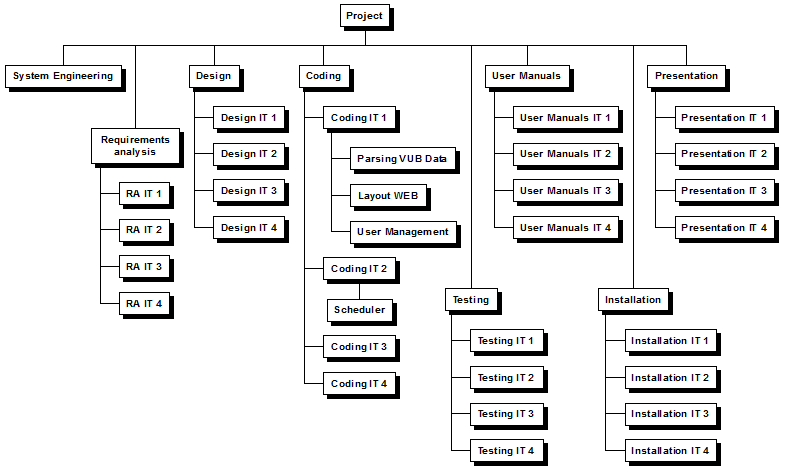
\includegraphics[width = \textwidth]{ManagerialProcess/WBSChart.png}
    \caption{Work breakdown structure.}
	\label{fig:workbreakdownstructure}
\end{figure}
Voor de eerste iteratie is de work breakdown structure weergegeven in figuur \ref{fig:wbsIteratie1}.
\begin{figure} [H]
	\centering
	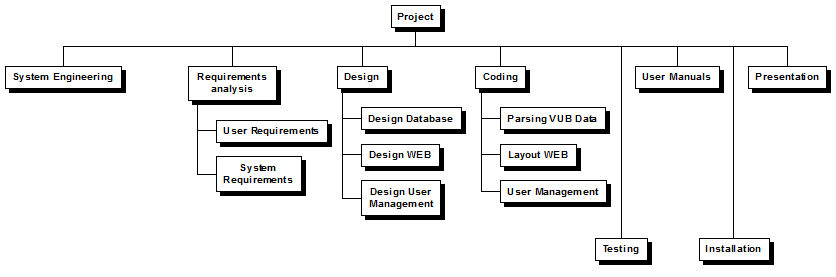
\includegraphics[width = \textwidth]{ManagerialProcess/WBSChartIteratie1.png}
	\caption{Work breakdown structure van iteratie 1.}
	\label{fig:wbsIteratie1}
\end{figure}
In de volgende versies van de SPMP zullen de work breakdown structures van de volgende iteraties worden weergegeven.
\subsection{Planning}
In tabel \ref{tab:ActivityDependenciesIteratie1} is een overzicht weergegeven van de verschillende activiteiten gedurende iteratie 1. Hierbij zijn ook de afhankelijkheden weergegeven tussen deze activiteiten. Op basis van deze tabel kunnen we een Gantt chart opstellen en het kritisch pad bepalen.
\begin{table} [H]
	\centering
	\caption{Activiteiten van de eerste iteratie en afhankelijkheden.}
	\begin{tabular} {l|l|c|c}
		Activiteit ID & Activiteit Naam & Tijdsduur (in dagen) & Afhankelijkheden \\
		\hline
		1 	& System Engineering 		& 28 & \\
		2 	& Requirements Analysis 	& 21 & \\
		2.1 & User Requirements 		& 10 & \\
		2.2 & System Requirements 		& 11 & 2.1 \\
		3 	& Design 					& 5 & 2 \\
		3.1 & Design User Management 	& 5 & \\
		4 	& Coding 					& 21 & \\
		4.1 & Infrastructure onderzoeken & 7 & 2\\
		4.2 & User Management			& 14 & 3, 4.1  \\
		4.2.1 & Frond End 		 		& 14 & \\
		4.2.2 & Back End				& 14 & \\
		5 	& Testing 					& 7 & 4.2 - 7 dagen \\
		6 	& User manuals 				& 3 & 4 \\
		7 	& Installation 				& 1 & 5,6 \\
		8 	& Presentation 				& 3 & 7	
	\end{tabular}
	\label{tab:ActivityDependenciesIteratie1}
\end{table}
Op basis van tabel \ref{tab:ActivityDependenciesIteratie1} bekomen we de Gantt chart voor iteratie 1 weergegeven in figuur \ref{fig:GantChartIT1}. Het kritisch pad is weergegeven in het rood. Hierbij is nog rekening met extra constraints:
\begin{itemize}
	\item Het project is gestart op 15 oktober 2013.
	\item De activiteit ``Requirements Analysis'' kan niet vroeger beginnen dan 24 oktober 2013.
	\item De activiteit ``Installation'' mag niet later eindigen dan 13 december 2013 (zie tabel \ref{tab:kalender}).
	\item De activiteit ``Presentation'' mag niet later eindigen dan 18 december 2013 (zie tabel \ref{tab:kalender}).
\end{itemize}
\begin{figure} [H]
	\centering
	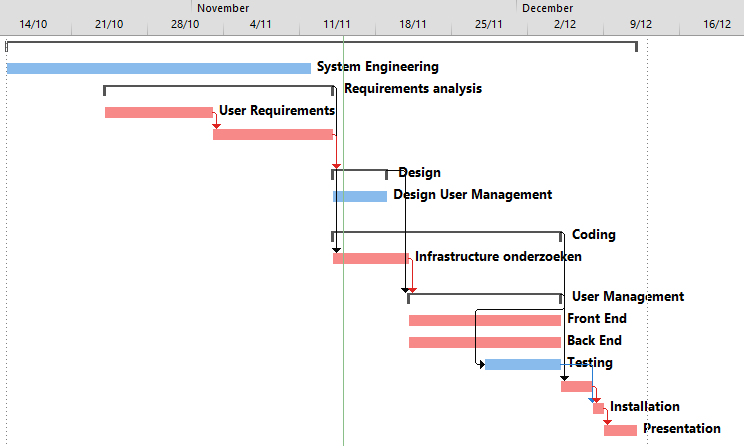
\includegraphics[width = \textwidth]{ManagerialProcess/GanttChartIT1.png}	
	\caption{Gantt chart voor iteratie 1.}
	\label{fig:GantChartIT1}
\end{figure}
Op figuur \ref{fig:GantChartIT1} is er te zien dat er nog enkele dagen marge zijn op het einde van iteratie 1. Het kritisch pad mag dus enkele dagen vertraging oplopen.
%\subsection{Middelen}
%This subclause of the SPMP shall provide a detailed itemization of the resources allocated to each major work activity in the project work breakdown structure. Resources shall include the numbers and required skill levels of personnel for each work activity. Resource allocation may include, as appropriate, personnel by skill level and factors such as computing resources, software tools, special testing and simulation facilities, and administrative support. A separate line item should be provided for each type of resource for each work activity. A summary of resource requirements for the various work activities should be collected from the work packages of the work breakdown structure and presented in tabular form.
%Voor de design-activiteiten zal er gebruik worden gemaakt van een UML Designer \footnote{De specifieke tool die we gaan gebruiken is nog onder overleg.}. Het coderen zal gebeuren in Eclipse. 

\section{Controle plan}
\subsection{Requirements controle} \label{RequirementsControlPlan}
Op de website van het team \cite{portalWebsite} zal er een pagina beschikbaar zijn die het mogelijk maakt om zaken te rapporteren, en veranderingen te controleren met betrekkeing tot de SRS.
\\
\\
Er zal een requirements dashboard beschikbaar zijn die een overzicht weergeeft van alle requirements en hun status per iteratie (done, busy, planned, deferred, ... ). Hierbij worden telkens de belangrijkste statistieken per requirement weergegeven (percentage afgewerkt indien bezig, duurtijd implementatie indien klaar, aantal unit tests, ... ).

\subsection{Planning controle}
Voor het opvolgen en schatten van de planning zal ook gebruik worden gemaakt van de website \cite{portalWebsite}. Door gebruik te maken van een eigen implementatie beschikken we over voldoende flexibiliteit. Bovendien is bijvoorbeeld het gebruik van Microsoft Project \cite{MicrosoftProject} niet bevorderend voor het gebruik in teamverband. Door alles gecentraliseerd op de website te plaatsen kan elk teamlid gemakelijk aan de meest recente project gegevens.

\subsection{Budget controle}
Op de website van het team \cite{portalWebsite} zal er gebruik gemaakt worden van een time tracking tool die het mogelijk maakt een gedetailleerd logboek bij te houden van de reeds uitgevoerde activiteiten. Op basis hiervan kunnen we dan de ``kost'' berekenen van het project. 
\\
\\
De tijdsregistratie wordt uitgevoerd bij het be\"{e}ndigen van elke werkdag. Hierbij wordt telkens opgegeven aan welke activiteit men gewerkt heeft (een overzicht van de verschillende activiteiten bevindt zich in sectie \ref{sec:workplan}).

\subsection{Kwaliteitscontrole}
Ook de kwaliteit zal opgevolgd worden met behulp van de website. De quality assurance leader zal verantwoordelijk zijn voor de kwaliteitspagina op de website.

\subsection{Rapportering} \label{sec:rapportering}
In tabel \ref{tab:kalender} worden de deliverables voor dit project weergegeven. Hierrond worden volgende afspraken gemaakt:
\begin{itemize}
\item Alle documenten en source code (inclusief unit tests) worden per mail aangeleverd als een enkele zipfile, met als naam se2-iterM, waarbij M het nummer van de iteratie is (voor eerste versie van documenten geldt M = 0). De aanlevering gebeurt ten laatste voor 9u00 ’s ochtends op de dag van de deadline (zie tabel \ref{tab:kalender}).
\item Alle documenten en source code worden worden overeenkomstig getagd/gebranchd (se2-iterM) in de GitHub repository.
\item Andere artefacten (zoals executables) worden apart aangeleverd (direct, of via een link, in de opleveringsmail) en vermelden duidelijk de overeenkomstige iteratie in de bestandsnaam.
\item De mail van de oplevering bevat een bondig overzicht (lijstje) van wat er precies opgeleverd
wordt.
\end{itemize}
Voor het verspreiden van de resultaten zal ook gebruik worden gemaakt van de website. 
\begin{itemize}
\item Opgeleverde documenten, source code en andere artefacten moeten publiekelijk en overzichtelijk beschikbaar zijn.
\item Het opleveren van documenten en code per iteratie houdt in dat ten laatste op die welbepaalde dag (zie tabel \ref{tab:kalender}) de site ook up-to-date wordt gebracht.
\end{itemize}
Een presentatie duurt een half uur per groep en wordt ingevuld door 2 sprekers. Alle groepsleden moeten minimum \'{e}\'{e}n keer presenteren. De volgende zaken worden besproken of gedemonstreerd:
\begin{itemize}
\item een demo van de toegevoegde functionaliteit ten opzichte van de vorige iteratie
\item analyse van de ontmoete obstakels en de genomen beslissingen
\item bespreking van de functionaliteiten die aan bod zullen komen in de volgende iteratie
\item bespreking van eventuele obstakels, risico’s, etc. in de volgende iteratie
\item overzicht van de architectuur en design van de applicatie
\item bespreking van de statistieken zoals de tijd per taak en per persoon en van de eventuele vertragingen (plus oplossingen om deze zo klein mogelijk te houden en te vermijden in de toekomst)
\end{itemize}

\subsection{Metriek verzamelingsplan}
Metrieken zullen verzameld worden met behulp van de Eclipse Metrics Plugin \cite{EclipseMetricsPlugin}. Er zullen metrieken op methodenniveau en klassenniveau verzameld worden. Op methodenniveau verzamelen we volgende metrieken:
\begin{enumerate}
	\item 
		Cyclomatic Complexity.
		\\
		\\
		Deze metriek geeft een indicatie van het aantal `lineaire' segementen in een methode (m.a.w. stukken code met geen branches). Dit kunnen we onder andere gebruiken om het aantal tests te bepalen om volledige dekking te krijgen. Het geeft ook een indicatie van de complexiteit van de methode.
		
	\item 
		Aantal statements
		\\
		\\
		Om de grootte van de methode te onderhouden, maken we gebruik van het aantal statements binnen een methode. Deze metriek is robuuster dan het aantal lijnen code vermits deze onafhankelijk is van de gebruikte programmeerstijl.
	\item
		Aantal levels.
		\\
		\\
		Deze metriek geeft het maximaal aantal geneste lagen in een methode. Een hoog aantal levels geeft aan dat we te maken hebben met een complexe  methode. Deze methoden kunnen vereenvoudigd worden door het extraheren van verscheidene private methoden.
	
	\item
		Aantal lokale variabelen in de scope.
		\\
		\\
		Deze metriek geeft het maximaal aantal lokale variable dat zich in de scope bevindt gedurende elk mogelijk punt in de methode. Een groot aantal wijst op complexe methoden.
	\item
		Aantal parameters.
		\\
		\\
		Deze metriek bevat het aantal parameters dat doorgegeven wordt aan een methode. Een te hoog aantal parameters wijst erop dat er te weinig gebruik gemaakt wordt van klassen.
	
	\item 
		Feature envy
		\\
		\\
		Deze metriek geeft aan in welke mate de methode ge\"{i}terreseerd is in methoden en attributen van andere klassen. Wanneer deze metriek een hoge waarde heeft, is het beter de methode te verplaatsen naar de klasse waarvan het het meest gebruik maakt. Wanneer dit gedrag slechts deels door een methode wordt bepaald, is het aangewezen om dit deel van de methode te verplaatsen (indien mogelijk).
		\\
		\\
		Voor de berekening gaan we als volgt te werk. Zij $m$ de methode waarvoor we de ``feature envy'' willen berekenen. We nemen dan $F_{c}$ de verzameling van features dat gebruikt worden door $m$ in klasse $c$. Verder is $c_{m}$ de klasse in welke de methode $m$ gedefinieerd is. We defini\"{e}ren dan de feature envy als:
		$$ FE = \max_{c \neq c_{m}} (|F_{c}|) - |F_{c_{m}}| $$
		Wanneer $FE > 0$ betekent dat de methode $m$ meer features gebruikt van een andere klasse. De klassenstructuur moet dan herzien worden. 

\end{enumerate}
Op klassenniveau verzamelen we volgende metrieken:
\begin{enumerate}
	\item 
		Efferent Couplings.
		\\
		\\
		In deze metriek wordt er gemeten hoeveel andere klassen de huidige klasse kent. Een hoog aantal koppelingen is nadelig voor de betrouwbaarheid van de code vermits het afhankelijk is van verscheidene types. Door de klasse op te delen in verscheidene deelklassen, kunnen we het aantal koppelingen naar omlaag brengen.
	\item
		Aantal attributen.
		\\
		\\
		Deze metriek meet het aantal attributen in een klasse. Bij een groot aantal attributen moet er nagegaan worden of er verscheidene attributen kunnen gegroepeerd worden in deelklassen.
	
	\item
		Complexiteit
		\\
		\\
		Deze metriek wordt berekend door de som te nemen van de Cyclomatic Complexities van de verschillende methoden die zich in deze klasse bevinden. Deze stelt dus de complexiteit voor van de gehele klasse.
		
	\item 
	{
		Cohesie tussen de verschillende methodes.
		\\
		\\
		De cohesie tussen de verschillende methoden in \'{e}\'{e}n enkele klasse is een belangrijk concept bij object georienteerd programmeren. De cohesie geeft aan of de klasse \'{e}\'{e}n of meerdere abstracties voorstelt. Indien \'{e}\'{e}n klasse meerdere abstracties voorstelt, moet deze opggesplitst worden in meerdere klassen waarbij elke klassen \'{e}\'{e}n abstractie voorstelt.
		\\
		\\
		Wij zullen de Henderson-Sellers metriek gebruiken \cite{HendersonSellers}. Om deze te berekenen voeren we volgende variabelen in: 
		$$ M = \{ m | \text{m is methode van de klasse} \} $$
		$$ F = \{ f | \text{f is een veld van de klasse} \} $$
		$$ r : F \rightarrow \mathbb{N} $$
Hierbij berekent $r(f)$ het aantal methoden dat veld $f$ aanroept. Vervolgens defini\"{e}ren we ook $\bar{r}$ als het gemiddelde van $r(f)$ over $F$. De Henderson-Seller metriek wordt dan berekent als:
		$$ HS = \frac{\bar{r} - |M|}{1 - |M|} $$
		Hoe lager de waarde, hoe beter de cohese tussen de verschillende methoden.
	} %TODO eventueel referentiewaarde en verklaren vanuit formule
\end{enumerate}
De Eclipse Metrics Plugin verzamelt automatisch metrieken bij elk compile process (eens geconfigureerd). Deze worden dan geexporteerd naar een XML-file die vervolgens wordt ingelezen door de website.
\\
\\
Verzamelde metrieken zullen op de webpagina van het team gevisualiseerd worden. De metrieken worden verzameld tijdens de activiteiten waar er gecodeerd wordt. Bij de start van het coderen zullen er wekelijks metrieken verzameld worden. In de laatste week van coderen worden er dagelijks metrieken verzameld, hierdoor kan er refactoring plaatsvinden die de kwaliteit van de code verhoogt.

\section{Risico management plan} \label{sec:risicoManagementPlan}
In deze paragraaf zullen de verschillende risico's verbonden aan dit project besproken worden. In paragraaf \ref{sec:riskPriority} zullen deze risico's gepriotiseerd worden. Om de risico's te kunnen prioritiseren zullen we gebruiken maken van 3 parameters:
\begin{itemize}
	\item 
		De kans $p$ waarmee dit risico kan voorkomen. Hierbij is $ p \in \{1, 2, \ldots , 10\} $. Verder betekent $p = 1$ dat het risico niet kan voorkomen en $p = 10$ dat het risico met zekerheid voorkomt.
	\item 
		De impact $i$ op het project wanneer het risico werkelijkheid wordt. Hierbij is $ i \in \{1, 2, \ldots , 10\} $. Verder betekent $i = 1$ een impact op het project die minimaal is en $i = 10$ een impact die maximaal is.
	\item 
		De kost $c$ die het risico heeft op het project om het probleem op te lossen. Hierbij is $ c \in \{1, 2, \ldots , 10\} $. Hierbij betekent $c = 1$ een lage kostprijs, terwijl $c=10$ een hoge kostprijs betekent. Bij een hoge kostprijs zal de prioriteit van het risico lager gesteld worden, vermits het dan beter kan zijn om pas het risico weg te werken wanneer het voorkomt. Hiermee worden grote onnodige kosten vermeden.
		
\end{itemize}
\subsection{Project risico's}
\subsubsection{Niet-realistische Planning}
In paragraaf \ref{sec:ProjectStartPlan} is de werkduur geschat met het COCOMO I-model. Hier werd reeds duidelijk dat de geschatte tijdsduur enorm hoog ligt. Dit zorgt voor een grote druk op de planning.
\\
\\
Om de vooropgestelde deadlines (zie tabel \ref{tab:kalender}) te bereiken dient men dus voldoende tijd vrij te maken. Het zwaartepunt van het academiejaar van de verschillende groepsleden ligt bij de meeste groepsleden in het eerste semester. Het grootste risico in verband met planning ligt dus vooral bij de eerste iteratie. Dit kan het best vermeden worden door gebruik te maken van interne deadlines en de progressie op te volgen tijdens de wekelijkske teammeetings.
\\
\\
We karakteriseren dit risico m.b.v. volgende parameters:
\begin{align*}
	p &= 8\\
	i &= 8\\
	c &= 2
\end{align*}

\subsubsection{Communicatieprobleem}
Bij een team van zeven personen is communicatie essentieel. Indien er geen bijzondere maatregelen worden genomen, zal deze snel verkeerd lopen.
\\
\\
Als oplossing hiervoor wordt er reeds een mailinglijst aangeleverd door VUB. Omdat wij deze niet overzichtelijk genoeg vinden, hebben wij zelf een communicatieplatform ontwikkeld op onze website. De werking verloopt als een blog waarbij de teamleaden een bericht kunnen plaatsen en vervolgens hierop kunnen reageren. Bij elk nieuw bericht worden de teamleden van een notificatie voorzien.
\\
\\
De implementatie hiervan is niet triviaal en vraagt de nodige investering. Wij verwachten echter dat de ``return on investment'' groot zal zijn. Samengevat:
\begin{align*}
	p &= 10\\
	i &= 8\\
	c &= 8
\end{align*}

\subsubsection{Meningsverschillen}
Bij het werken in teamverband is het onvermijdelijk dat er meningsverschillen optreden tussen verscheidene groepsleden. We maken een onderscheid tussen volgende menigsverschillen:
\begin{itemize}
	\item Functioneel: Meningsveschillen waarvan de uitkomst bepalend is voor de uiteindelijke werking van het programma.
	\item Niet-functioneel: Meningsverschillen waarvan de uitkomst niet bepalend is voor de uiteindelijke werking van het programma. Bijvoorbeeld de communicatiemethode, meningsveschillen over interne deadlines, persoonlijke conflicten tussen teamleden, ...
\end{itemize}
Verder kunnen we ook nog onderscheid maken tussen kleine en grote meningsverschillen. Al deze types worden opgelost op een verschillende manier, weergegeven in tabel \ref{tab:meningsverschillen}. De `kost' voor het oplossen van het risico is dus minimaal.
\begin{table} [H]
	\centering
	\caption{Oplossingen voor de verschillende meningsconflicten.}
	\begin{tabular} {l|ll}
					& Functioneel 								& Niet-functioneel \\
			\hline
			Groot 	& Meeting met team, vervolgens stemming		& Behandeld door de verantwoordelijke \\ 
			& & van dit onderwerp \\
			Klein 	& Project Manager							& Behandeld door de verantwoordelijke \\
			& & van dit onderwerp
	\end{tabular}
	\label{tab:meningsverschillen}
\end{table}
We karakteriseren dit risico m.b.v. volgende parameters:
\begin{align*}
	p &= 10\\
	i &= 3\\
	c &= 2
\end{align*}

\subsection{Technische risico's}
\subsubsection{Gebrek aan ervaring in de implementatie-technologie}
Hiervoor wordt er gekeken naar de programmeertalen die gebruikt worden tijdens dit project (zie sectie \ref{sec:languages}). Een overzicht van de aanwezige kwaliteiten is zichtbaar in tabel \ref{tab:skilllevel}. Wat opvalt is dat er van elks kwaliteiten aanwezig zijn, maar er zijn ook de nodige aandachtspunten. Zo is bijvoorbeeld de ervaring in Java en JavaScript beperkt.

\begin{table} [htbp]
	\centering
  	\caption{Ervaring van de verschillende teamleden.}
    \begin{tabular}{c|ccccl}
  		  	& Java 	& JavaScript & HTML \textbackslash CSS 		& SQL 	& Opmerkingen \\
  		  	\hline
  		  	Christophe & -	& ++ 		& ++ 		& ++ & \shortstack{ Reeds ervaring opgedaan \\ in de bedrijfswereld} \\
  		  	Youri & + & - & - & ++ & \shortstack{Voorkeur voor logica, \\ A.I. en modeleren.} \\
  		  	Nicolas & + & - & + & ++ & Voorkeur voor back end \\
  		  	Tim & - & - & + & ++ & \shortstack{Reeds ervaring in C++ en \\ andere programmeerprojecten} \\
  		  	Sam & + & - & + & ++ & \\
  		  	Fernando & - & - & + & ++ & Voorkeur voor design \\
  		  	Pieter & ++ & + & + & + & \shortstack{Reeds ervaring opgedaan \\ in de bedrijfswereld}
    \end{tabular}
  	\label{tab:skilllevel}
\end{table}
Omdat de implementatie-technologie opgelegd wordt, is het gebruik maken van andere frameworks, programmeertalen, ... geen optie. Hierdoor zullen we gebruik maken van workshops. Hiermee gaan we de ervaringen van de verschillende teamleden op elkaar overbrengen. Een workshop wordt georganiseerd door een teamlid die zijn kennis en ervaringen over een bepaalt framework, programmeertaal, ... uiteenzet gedurende 30 \`{a} 60 minuten. Volgende workshops zijn reeds gepland:
\begin{itemize}
	\item GitHub (door Christophe)
	\item Java (door Pieter)
\end{itemize}
Doordat we gebruik maken van korte workshops, zou de invloed van deze workshops op de planning minimaal zijn. We karakteriseren dit risico m.b.v. volgende parameters:
\begin{align*}
	p &= 8\\
	i &= 8\\
	c &= 4
\end{align*}

\subsubsection{Gebrekkige performantie}
Het hoofddoel van dit project is het maken van een scheduler. Het is uiteraard gewenst dat het schedulen vlot verloopt. Vanwege de complexiteit van dit onderwerp zal er ook de nodige aandacht besteedt moeten worden aan de performantie van de scheduler.
\\
\\
Dit zal gemonitored worden met behulp van benchmarks. Indien er tekortkomingen ontdekt worden, zullen de nodige optimalisaties moeten doorgevoerd worden aan de scheduler. We karakteriseren dit risico m.b.v. volgende parameters:
\begin{align*}
	p &= 7\\
	i &= 2\\
	c &= 7
\end{align*}

\subsubsection{Support voor meerdere browsers}
Uit ervaring weten we dat Internet Explorer soms voor compatibiliteitsproblemen zorgt. Het is niet nodig om dit risico op voorhand te elimineren. Op voorhand alle compabiliteitsproblemen opzoeken bij verschillende browsers zou een immens werk zijn. Wanneer bij het testen duidelijk wordt dat er problemen optreden in een bepaalde browser, moet dit opgelost worden d.m.v. de benodigde documentatie op te zoeken op internet. We karakteriseren dit risico m.b.v. volgende parameters:
\begin{align*}
	p &= 7\\
	i &= 4\\
	c &= 10
\end{align*}

\subsubsection{Merge conflicten}
Bij het werken met de GitHub repository zijn merge conflicten nooit verweg. Door het werken met forking en pull requests vermijden we echter deze conflicten en zorgen we voor een goed beheer van onze GitHub repository. Het implementeren van forking en pull requests vergt echter enig opzoekwerk waardoor de kost hoog ligt. Het beheer van de GitHub repository wordt verder besproken in het SCMP (zie paragraaf \ref{SoftwareConfigurationManagementPlan}.
\begin{align*}
	p &= 10\\
	i &= 5\\
	c &= 7
\end{align*}

\subsubsection{Bugs}
Bugs zijn onvermijdelijk in een programma. De procedure voor bugs af te handelen wordt besproken in het problem resolution plan (zie paragraaf \ref{sec:ProblemResolutionPlan}). Dit risico wordt gekarakteriseerd met volgende parameters:
\begin{align*}
	p &= 10\\
	i &= 7\\
	c &= 3
\end{align*}

\subsection{Bedrijfsrisico's}
\subsubsection{Ontwikkelen van de verkeerde functionaliteit}
Het ontwikkelen van verkeerde functionaliteit is steeds een re\"{e}el risico. Doordat we gebruik maken van een iteratief development process, waarbij we bij elke iteratie werkende code opleveren, krijgen we geregeld feedback van de klant. Hierdoor kunnen we de requirements, indien nodig, bijsturen. Vermits we bij de start van elke iteratie een gedetailleerde planning opstellen, kunnen eventuele wijzigingen vlot verwerkt worden. We karakteriseren dit risico m.b.v. volgende parameters:
\begin{align*}
	p &= 6\\
	i &= 7\\
	c &= 4
\end{align*}

\subsection{Prioriteit van de verschillende risico's.} \label{sec:riskPriority}
Op basis van de 3 parameters $p$, $i$ en $c$ berekenen we de prioriteit $P$ van het risico \cite{SoftwareEngineeringAModernApproach}
$$ P = (11 - p)*(11 - i)*c$$
Vermits hoge waarden van $p$, $i$ en kleine $c$ belangrijker zijn, zijn de risico's met de kleinste waarden van $P$ het belangrijkste. Een (gesorteerd) overzicht is weergegeven in tabel \ref{tab:riskPriorityTabel}.
\begin{table} [H]
	\centering
	\caption{Prioriteit van de verschillende risico's.}
	\begin{tabular} {l|ccc|c}
		Risico & $p$ & $i$ & $c$ & $P$ \\
		\hline
		Bugs						& 10	& 7 	& 3		& 12 \\
		Meningsverschillen 			& 10	& 3		& 2		& 16 \\
		Niet-realistische planning 	& 8 	& 8 	& 2 	& 18 \\
		Communicatieprobleem		& 10	& 8		& 8		& 24 \\ 
		Gebrek aan ervaring 		& 8 	& 8 	& 4 	& 36 \\
		Merge conflicten			& 10	& 5		& 7		& 42 \\
		Verkeerde functionaliteit 	& 6 	& 7 	& 4 	& 80 \\
		Performantie 				& 7 	& 2 	& 7 	& 252 \\
		Browser support				& 7 	& 4 	& 10 	& 280
	\end{tabular}
	\label{tab:riskPriorityTabel}
\end{table}

%\section{Project closeout plan} niet.